\documentclass[12pt,a4paper]{article}
\usepackage[T2A]{fontenc}
\usepackage[utf8]{inputenc}
\usepackage[english,russian]{babel}
\usepackage{amsmath}
\usepackage{graphicx}
\usepackage{booktabs}
\usepackage[margin=22mm]{geometry}
\usepackage[unicode,hidelinks]{hyperref}

\title{Паспорт учебного проекта}
\author{Учебная группа}
\date{}

\begin{document}
\maketitle

\section{Задача}
Мы передаём учебный проект другой группе. Получатель должен понять,
как запустить работу, что разрешено использовать и в чём состоит результат.
Это пример оформления, а не отчёт о проведённом эксперименте.

\section{Модель}
Пусть $n_i$ --- число объектов категории $i$, а всего категорий $k$.
Доля категории при непустом наборе определяется как
\begin{equation}
    p_i = \frac{n_i}{\sum_{j=1}^{k} n_j},
    \qquad \sum_{j=1}^{k} n_j > 0.
    \label{eq:share}
\end{equation}
В формуле~\eqref{eq:share} знаменатель --- общее число объектов.
Если объектов нет, доли по этой формуле не определены.

\section{Что передаём}
На рисунке~\ref{fig:workflow} показан путь от исходника к читателю.
\begin{figure}[ht]
    \centering
    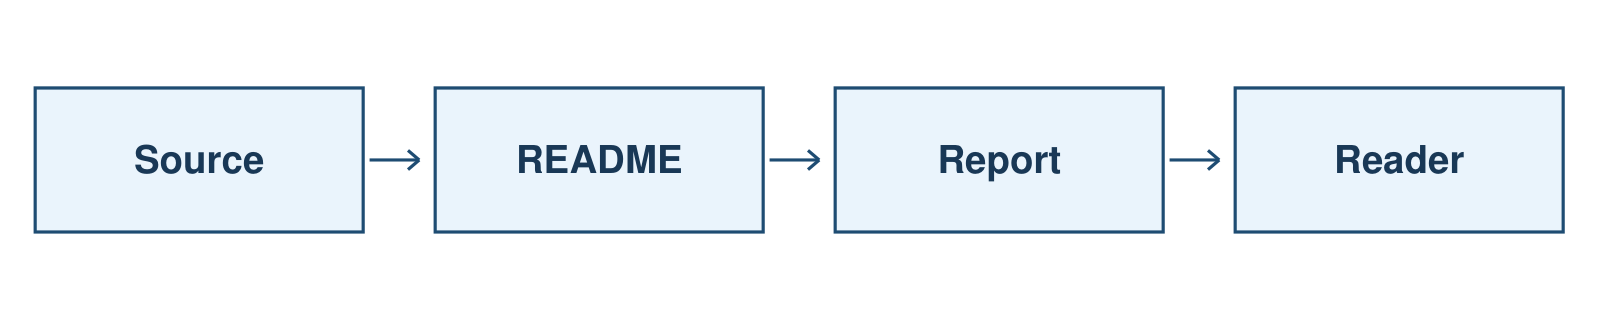
\includegraphics[width=\linewidth]{workflow.png}
    \caption{От исходника к понятному результату}
    \label{fig:workflow}
\end{figure}

\begin{center}
\begin{tabular}{ll}
\toprule
Файл & Назначение \\
\midrule
\texttt{README.md} & Инструкция пользователю \\
\texttt{report.tex} & Исходник технической записки \\
\texttt{report.pdf} & Собранный документ \\
\bottomrule
\end{tabular}
\end{center}

\end{document}
